\section{Trajectory}
\label{sec:Trajectory}
%%%%%%%%%%%%%%%%%%%%%%%%%%%%%%%%%%%%%%%%%%%%%%%%%%%%%%%%
\begin{figure}[h!]
\begin{center}
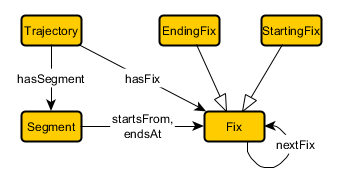
\includegraphics[width=.8\textwidth]{figures/trajectory}
\end{center}
\caption{Schema Diagram for the Trajectory Pattern. The visual notation is explained in Chapter \ref{chap:prelims}.}
\label{fig:Spatiotemporal}
\label{fig:Trajectory}
\end{figure}
\subsection{Summary}
\label{sum:Trajectory}
%%%%%%%%%%%%%%%%%%%%%%%%%%%%
I am some summary text.

%%%%%%%%%%%%%%%%%%%%%%%%%%%%%%%%%%%%%%%%%%%%%%%%%%%%%%%%
\subsection{Axiomatization}
\label{axs:Trajectory}
%%%%%%%%%%%%%%%%%%%%%%%%%%%%
\begin{align}
\textsf{Segment} &\sqsubseteq \mathord{=1}\textsf{startsFrom.Fix}\\
\textsf{Segment} &\sqsubseteq \mathord{=1}\textsf{endsAt.Fix} \\
\textsf{Segment} &\sqsubseteq \exists \textsf{hasSegment}^-\textsf{.Trajectory} \\
\textsf{startsFrom}^- \circ \textsf{endsAt} &\sqsubseteq \textsf{hasNext} \\
\textsf{hasNext} &\sqsubseteq \textsf{hasSuccessor} \\
\textsf{hasSuccessor} \circ \textsf{hasSucessor} &\sqsubseteq \textsf{hasSucessor} \\
\textsf{hasNext}^- &\equiv \textsf{hasPrevious} \\
\textsf{hasSuccessor}^- &\equiv \textsf{hasPredecessor} \\
\textsf{Fix} \sqcap \lnot\exists\textsf{endsAt}^-\textsf{.Segment} &\sqsubseteq \textsf{StartingFix} \\
\textsf{Fix} \sqcap \lnot\exists\textsf{startsFrom}^-\textsf{.Segment} &\sqsubseteq \textsf{EndingFix} \\
\textsf{Trajectory} &\sqsubseteq \exists\textsf{hasSegment.Segment} \\
\textsf{hasSegment} \circ \textsf{startsFrom} &\sqsubseteq \textsf{hasFix} \\
\textsf{hasSegment} \circ \textsf{endsAt} &\sqsubseteq \textsf{hasFix} \\
\exists \textsf{hasSegment.Segment} &\sqsubseteq \textsf{Trajectory} \\
\exists \textsf{hasSegment}^-\textsf{.Trajectory} &\sqsubseteq \textsf{Segment} \\
\exists \textsf{hasFix.Segment} &\sqsubseteq \textsf{Trajectory} \\
\exists \textsf{hasFix}^-\textsf{.Trajectory} &\sqsubseteq \textsf{Fix}
\end{align}

%%%%%%%%%%%%%%%%%%%%%%%%%%%%%%%%%%%%%%%%%%%%%%%%%%%%%%%%
\subsection{Explanations}
\label{exp:Trajectory}
%%%%%%%%%%%%%%%%%%%%%%%%%%%%
\begin{enumerate}
\item \textsf{Segment} \textsf{startFrom} exactly one \textsf{Fix}.
\item \textsf{Segment} \textsf{endsAt} exactly one \textsf{Fix}.
\item Existential: A \textsf{Segment} belongs to at least one \textsf{Trajectory}.
\item Role Chain: the concatenation of \textsf{startsFrom}$^-$ nad \textsf{endsAt} is \textsf{hasNext}.
\item Subproperty: \textsf{hasNext} is a subproperty to \textsf{hasSuccessor}.
\item Role Chain: \textsf{hasSuccessor} is transitive.
\item Inverse Alias.
\item Inverse Alias.
\item A \textsf{Fix} that is not where a segment ends is a \textsf{StartingFix}.
\item A \textsf{Fix} that is not where a segment starts is a \textsf{EndingFix}.
\item Existential: a \textsf{Trajectory} has at least one \textsf{Segment}.
\item Role Chain: the concatenation of \textsf{hasSegment} and \textsf{startsFrom} is \textsf{hasFix}.
\item Role Chain: the concatenation of \textsf{hasSegment} and \textsf{endsAt} is \textsf{hasFix}.
\item Scoped Domain: the domain of \textsf{hasSegment}, scoped by \textsf{Segment}, is \textsf{Trajectory}.
\item Scoped Domain: the domain of \textsf{hasSegment}$^-$, scoped by \textsf{Trajectory}, is \textsf{Segment}.
\item Scoped Domain: the domain of \textsf{hasFix}, scoped by \textsf{Segment}, is \textsf{Trajectory}.
\item Scoped Domain: the domain of \textsf{hasFix}$^-$, scoped by \textsf{Trajectory}, is \textsf{Fix}.
\end{enumerate}

%%%%%%%%%%%%%%%%%%%%%%%%%%%%%%%%%%%%%%%%%%%%%%%%%%%%%%%%
\subsection{Competency Question}
\label{cqs:Trajectory}
%%%%%%%%%%%%%%%%%%%%%%%%%%%%
\begin{enumerate}[CQ1.]
\item temporary item
\end{enumerate}

\newpage
%%%%%%%%%%%%%%%%%%%%%%%%%%%%%%%%%%%%%%%%%%%%%%%%%%%%%%%%
% End Section
%%%%%%%%%%%%%%%%%%%%%%%%%%%%%%%%%%%%%%%%%%%%%%%%%%%%%%%%
%%%%%%%%%%%%%%%%%%%%%%%%%%%%%%%%%%%%%%%%%%%%%%%%%%%%%%%%